\section{Results}
In our snapshot deduplication architecture, CDS is the key to achieve greater deduplication than
incremental backup solutions. Our basic assumption of CDS us that VM disks, especially OS disks,
have huge amount of data in common, and such common data can be represented by a relatively smaller data set
because of their high appearence frequency. As a result, the major portion of snapshot deduplication effect shall 
emerge from eliminating the duplication of such a small data set. In this section, we evaluate
the effectiveness of CDS using real user VM disks from our production VM cluster.

\subsection{Experiment Setup}
The data set we use is the same as described in previous section. 
We choose extreme binning and perfect deduplication to compare against.
In all experiments, our deduplication enforces 2MB fix-sized segment boundary, 
and uses TTTD algorithm to divide segment into 4KB variable-sized blocks.
For perfect deduplication and extreme binning, the whole snapshots are splitted
using TTTD with 4KB average size. The original extreme binning paper uses whole file
as the input unit, but that is way too big for our system. 
Thus we split image snapshot files into variable-sized segments base on the block hash list, 
using TTTD with average size of 2MB.

\subsection{OS Disk}
We extract the CDS of OS disks by counting the blocks that will appear in a VM's
block store if no CDS is involved in the deduplication process. The threshold is set to less than
1.5\%, which is quite sufficient to include the OS related data since their duplication is much
heavier than others. Then we use this CDS to run the deduplication process again.
Finally we extracted about 80GB of CDS data from 350 OS disk snapshots,
the corresponding CDS meta occupies 800MB in CDS cache.

\begin{figure}
  \centering
  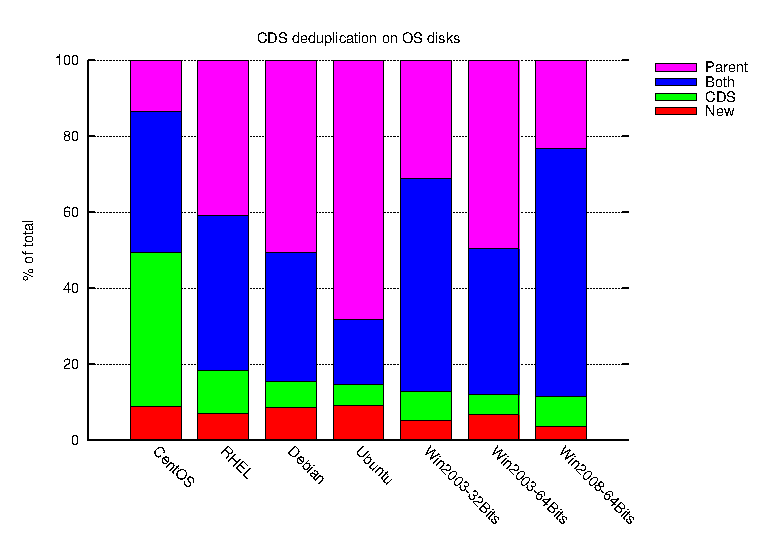
\epsfig{file=images/os_cds_sim.eps, height=2in, width=2.66in}
  \caption{CDS deduplication effect on OS disks}
  \label{fig:oscds}
\end{figure}

For each block, we tag it with one of the following:
\begin{itemize}
\item {New: this block cannot be deduplicated and thus write to block store.}
\item {CDS: this block is deduplicated by CDS.}
\item {Parent: this block is not found in CDS, but is found in parent snapshot's segment recipe.}
\item {Both: this block is both found in CDS and parent snapshot.}
\end{itemize}
As we can see from \ref{fig:oscds}, locality dominates.
This is because the interval between two snapshots is quite short due to our daily snapshot strategy. 
However, locality still doesn't work well on some of the OSes. But CDS, on the contrary,
finds a lot of duplicates that locality can't find, especially in a VM's first snapshot.

Combining all the VMs, we see the overall 7.4TB of data is reduced to 512GB. Extreme bining 
reduces this data set to 542GB, which is slightly worse. As a reference, perfect deduplication achieves
364GB in this experiment.

Overall, none of locality or CDS can solely work well, but by combining them together 
we get fairly good and stable deduplication ratio to all kind of OSes. If compare to all
incremental backup solutions, CDS can save addition 50\%+ of disk space because it greatly reduces
the cross-VM duplicates.

\subsection{Data Disk}
Figure \ref{fig:pd} shows the compression ratio of perfect deduplication at different data scales. 
Basically perfect deduplication would help us save 50\% of space on user data, 
regardless of scale. If we put all these unique data into CDS, we could achieve perfect deduplication, 
which is not affordable. So we need to see how much space saving of perfect 
deduplication can be achieved through a limit size CDS.
\begin{figure}
  \centering
  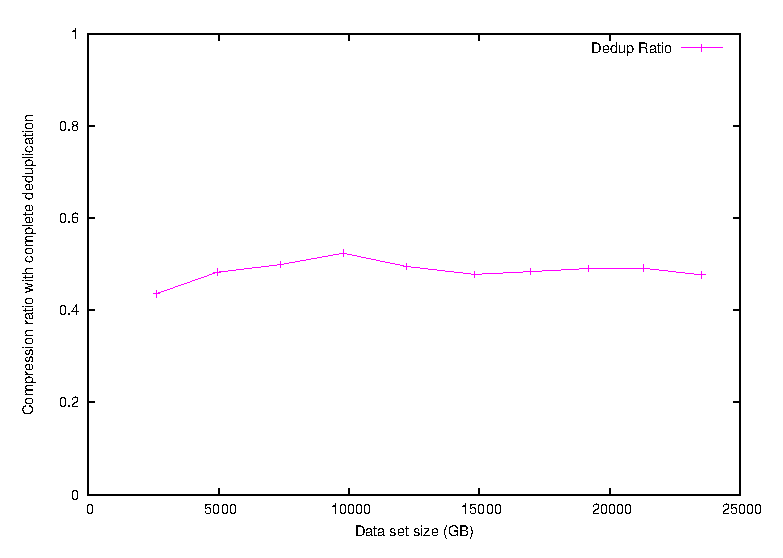
\epsfig{file=images/dedup_ratio.eps, height=2in, width=2.66in}
  \caption{Perfect deduplication on data disks}
  \label{fig:pd}
\end{figure}

We rank unique data blocks by their duplication count, 
and choose the hottest blocks as CDS. 
We define \emph{space saving ratio} as the space saving of CDS divide by 
perfect deduplication saving. Figure \ref{fig:datacdssize} shows the relationship between CDS size and space saving. 
It’s clear a very small amount of CDS data provides more than 50\% saving. 
But this effect decreases when more data are added to CDS. 
The lower bound of CDS space saving ratio is 50\%, which is very easy to accomplish. 

\begin{figure}
  \centering
  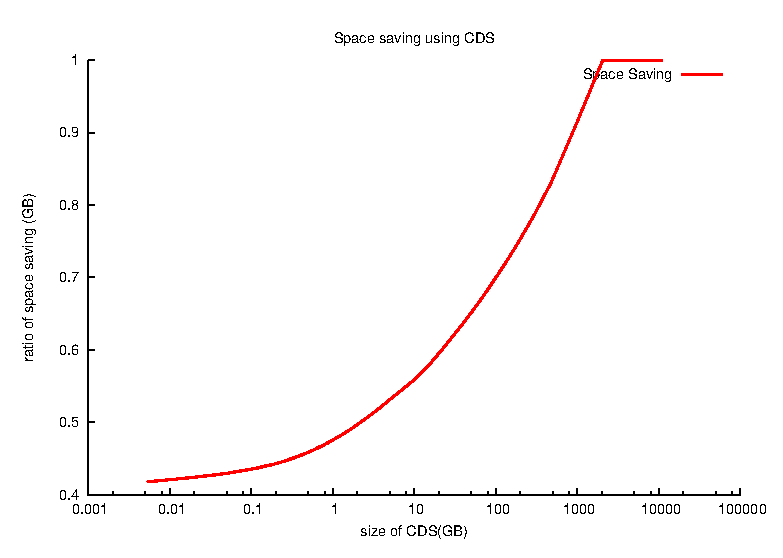
\epsfig{file=images/uniquedata-saving.eps, height=2in, width=2.66in}
  \caption{Size of CDS vesus space saving}
  \label{fig:datacdssize}
\end{figure}

The upper bound of CDS size is restricted by system memory resource.
Figure \ref{fig:datacds} shows how CDS space saving is affected by the system scale. 
In this experiment we first set out a goal of space saving ratio, 
then we watch how much data we need to put into CDS to achieve this goal.
From the graph we can see a 75\% saving goal lead to a stable ratio between 
CDS size and data size, which requires 0.01\% of data to be put in CDS.

Base on above data we can estimate the size of data CDS and its effect. 
Currently we prepared 500MB memory per machine to store CDS meta, then it can represent 50GB of data. 
If we assume each VM has 30GB of user data at runtime, and we host 25 VMs per machine, 
 maintain 10 snapshots per VM, each brings 10\% additional modified data. 
Thus the user data in snapshot system is 1.5TB per machine. So the upper bound of 
$CDS size/ Data size = 0.033$, which is sufficient for the 75\% saving goal.

\begin{figure}
  \centering
  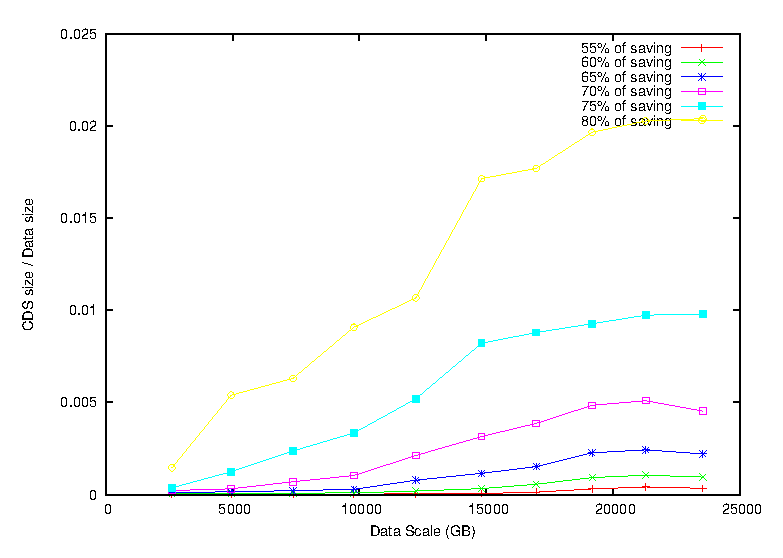
\epsfig{file=images/cds_scale.0.7.eps, height=2in, width=2.66in}
  \caption{CDS deduplication effect on data disks}
  \label{fig:datacds}
\end{figure}

Unlike the CDS of OS disks which is mainly composed of OS related data thus highly predictable, 
data disks is unpredictable because we cannot control what user can put in there. But we still
suspect that highly duplicated data in existing data are very likely to be duplicated again.
So we randomly pick 50 out of 1322 data disks as the new data, and use the rest as existing data
to extract CDS. Using 1.5\% as CDS threshold, we see the total 1198GB of new data is reduced by 
755.8GB, while perfect deduplication can reduce 1017.4GB. So 74.3\% of duplicate blocks are eliminated 
by pre-trained CDS, which is quite satisfiable.
